\section{Results}

\subsection{$P_0$ distribution choice}

Figure \ref{fig:P0_logprob} shows the effect of phoneme distribution choice on the log joint probability. It turns out that the choice does hardly influences the log joint probability at all.

\begin{figure}
  \centering
    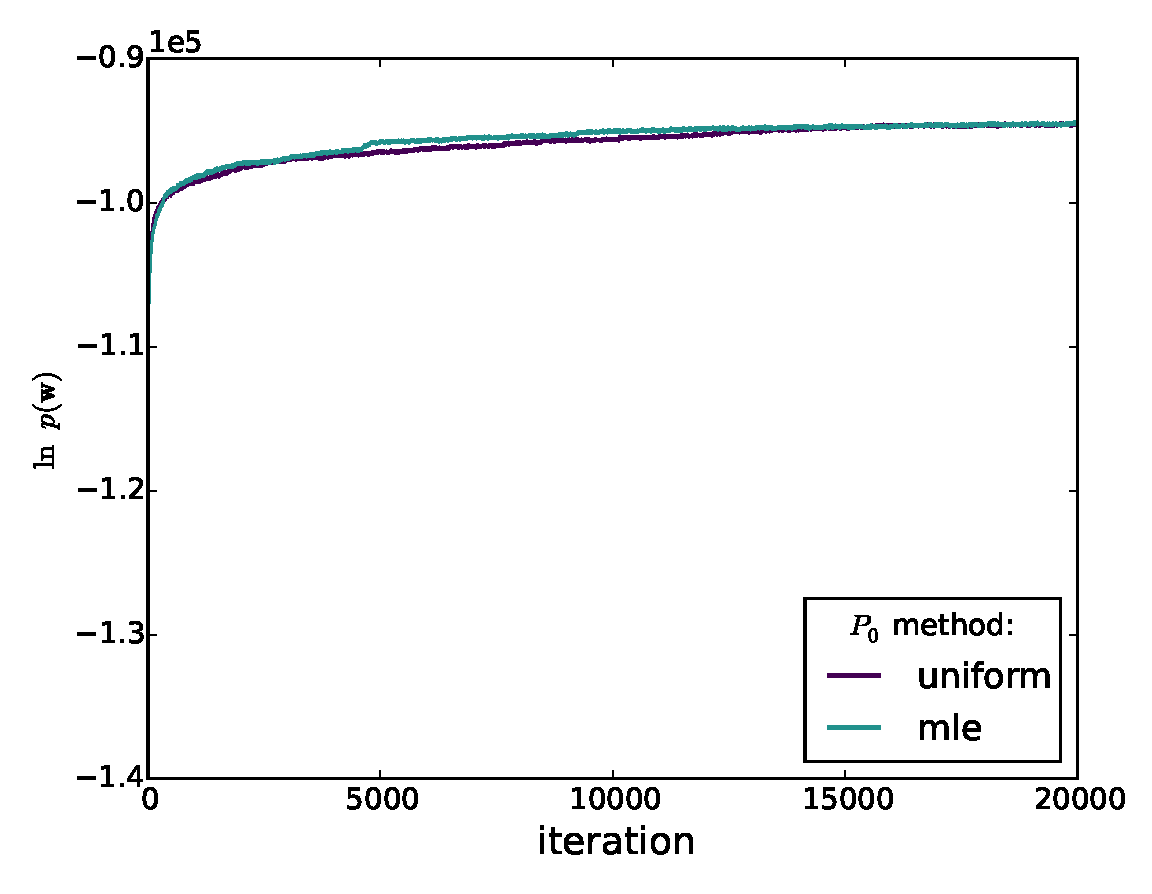
\includegraphics[width=0.75\textwidth]{images/P0_method-log_prob}
  \caption{The effect of phoneme distribution choice for $P_0$ on the log joint probability over time.}
  \label{fig:P0_logprob}
\end{figure}

\subsection{Gibbs sampling}

\subsubsection{Temperature regime}

Figure \ref{fig:temp_logprob} shows the effect of temperature regime on the log joint probability over time. We conclude that regime 2, which starts very low and increments the temperature by a small amount relatively often, leads to the highest log joint probability, both initially and after many iterations.

\begin{figure}
  \centering
    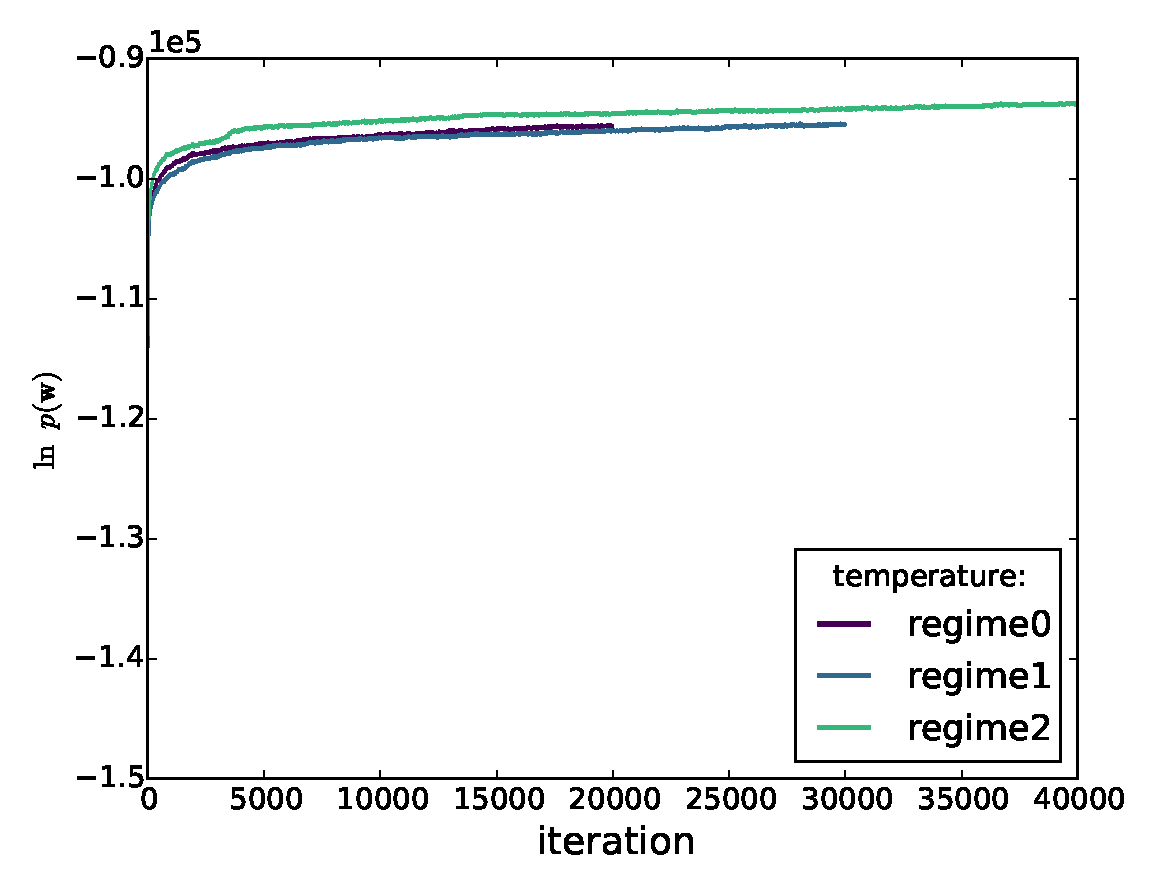
\includegraphics[width=0.75\textwidth]{images/temperature-log_prob}
  \caption{The effect of temperature regime on the log joint probability over time.}
  \label{fig:temp_logprob}
\end{figure}

\subsubsection{Initialisation strategy}

Figure \ref{fig:init_logprob} shows the effect of initialisation strategy on the log joint probability over time. It shows that not initialising the boundaries at all leads to the highest log joint probability, both initally and after many iterations.

\begin{figure}
  \centering
    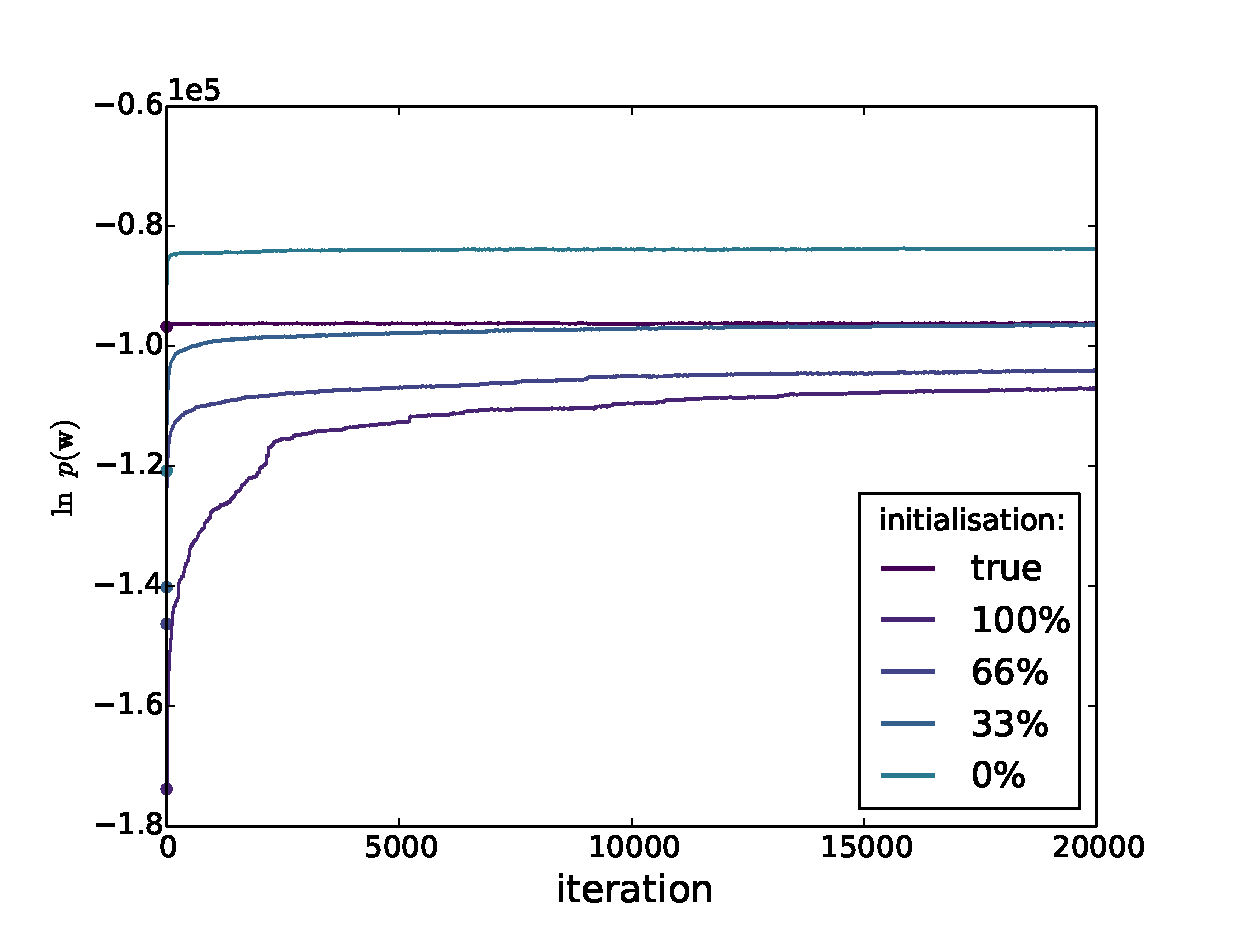
\includegraphics[width=0.75\textwidth]{images/initialisation-log_prob}
  \caption{The effect of initialisation strategy on the log joint probability over time.}
  \label{fig:init_logprob}
\end{figure}

\subsection{Model parameters}

Figure \ref{fig:model_parameters} shows the effect of different model parameter choices on retrieval quality, evaluated on words, boundaries and the lexicon. The effect is mostly visible at the lexicon level, favouring higher values for both $\alpha_0$ and $p_\#$, but it does not seem to affect the retrieval quality of the words and boundaries much.

\begin{figure}[!ht]
\begin{tabular}{cccc}
\subfloat[Precision for different values of $\alpha_0$]{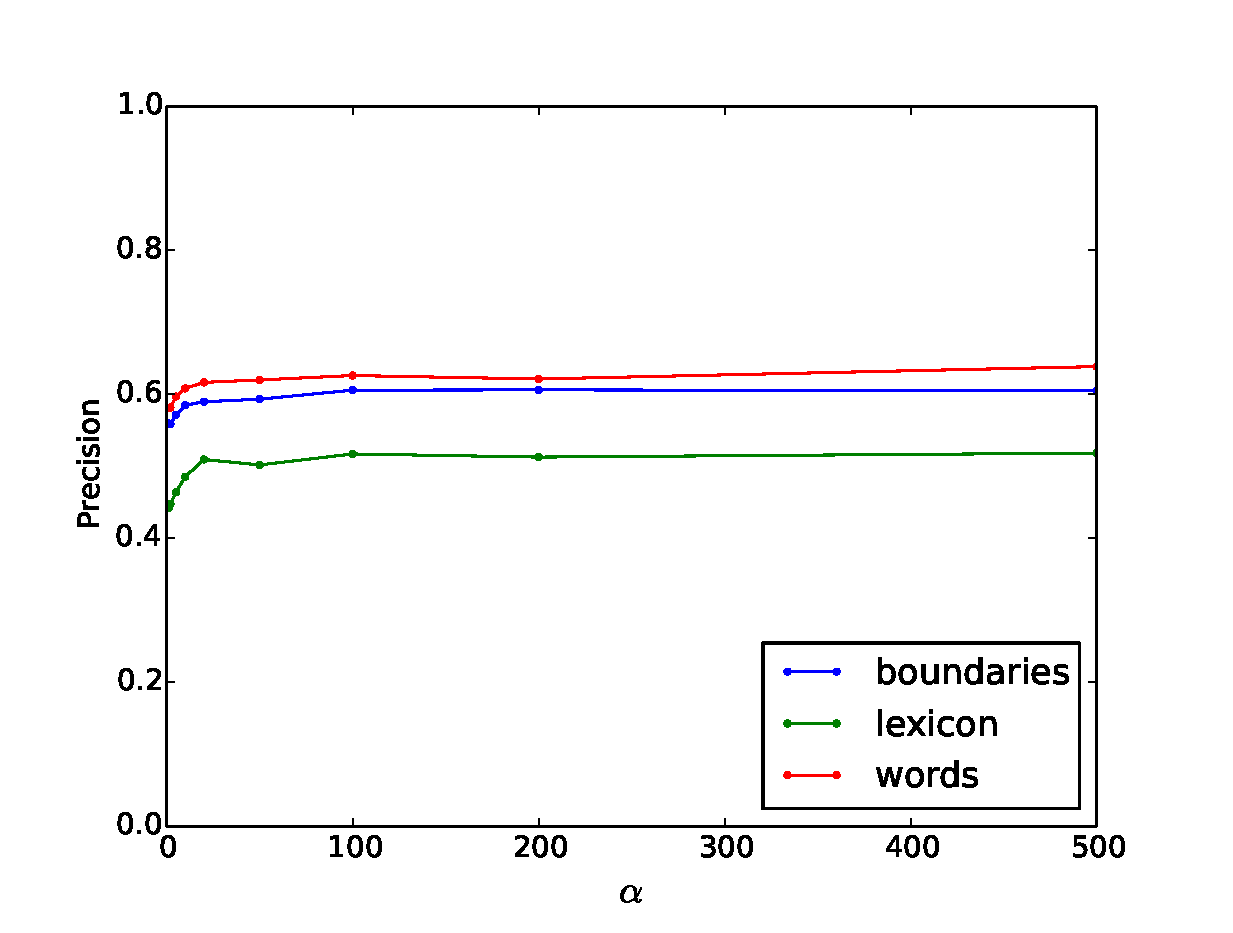
\includegraphics[width=0.47\linewidth]{images/alpha-precision}} &
\subfloat[Precision for different values of $p_\#$]{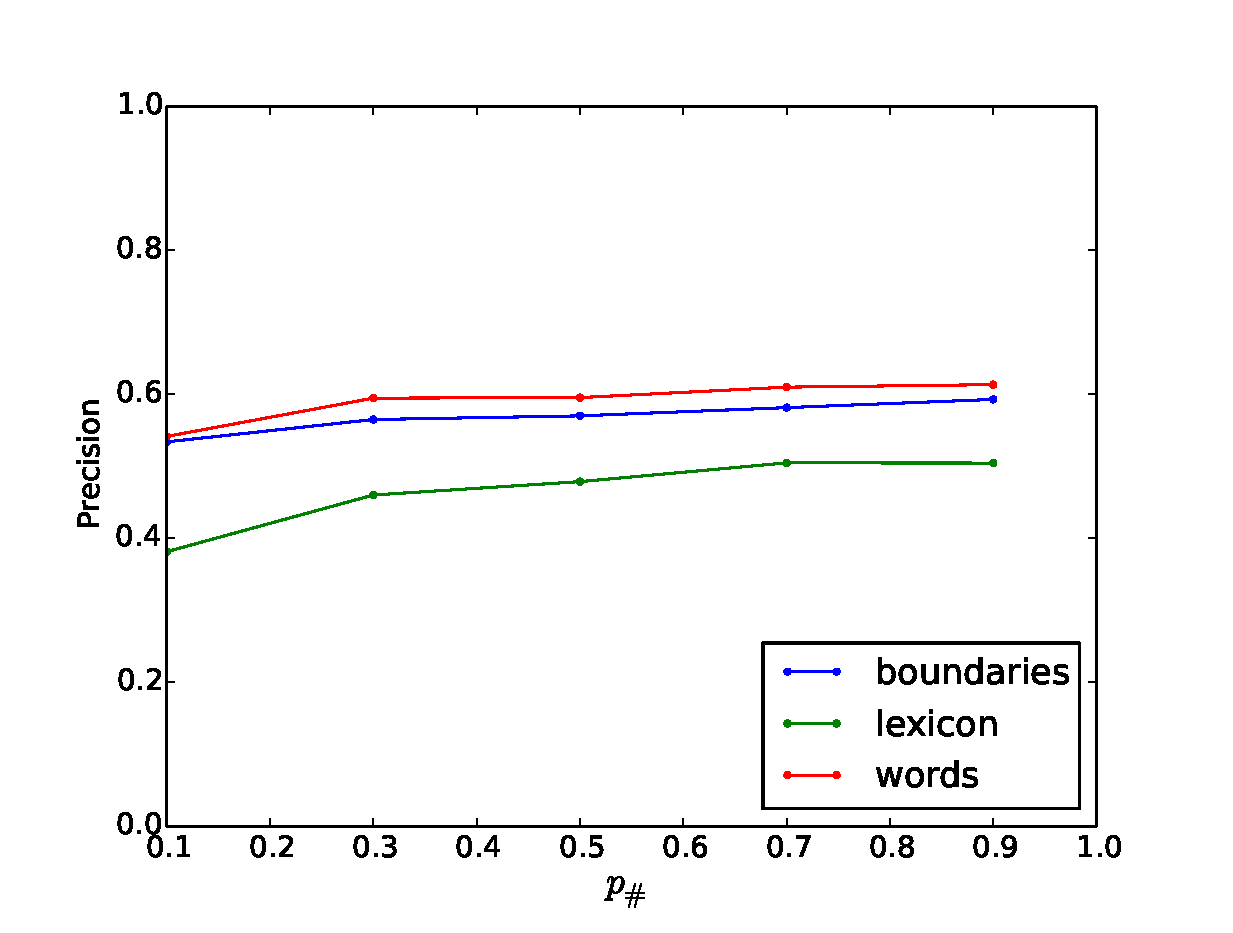
\includegraphics[width=0.47\linewidth]{images/p_dash-precision}} \\
\subfloat[Recall for different values of $\alpha_0$]{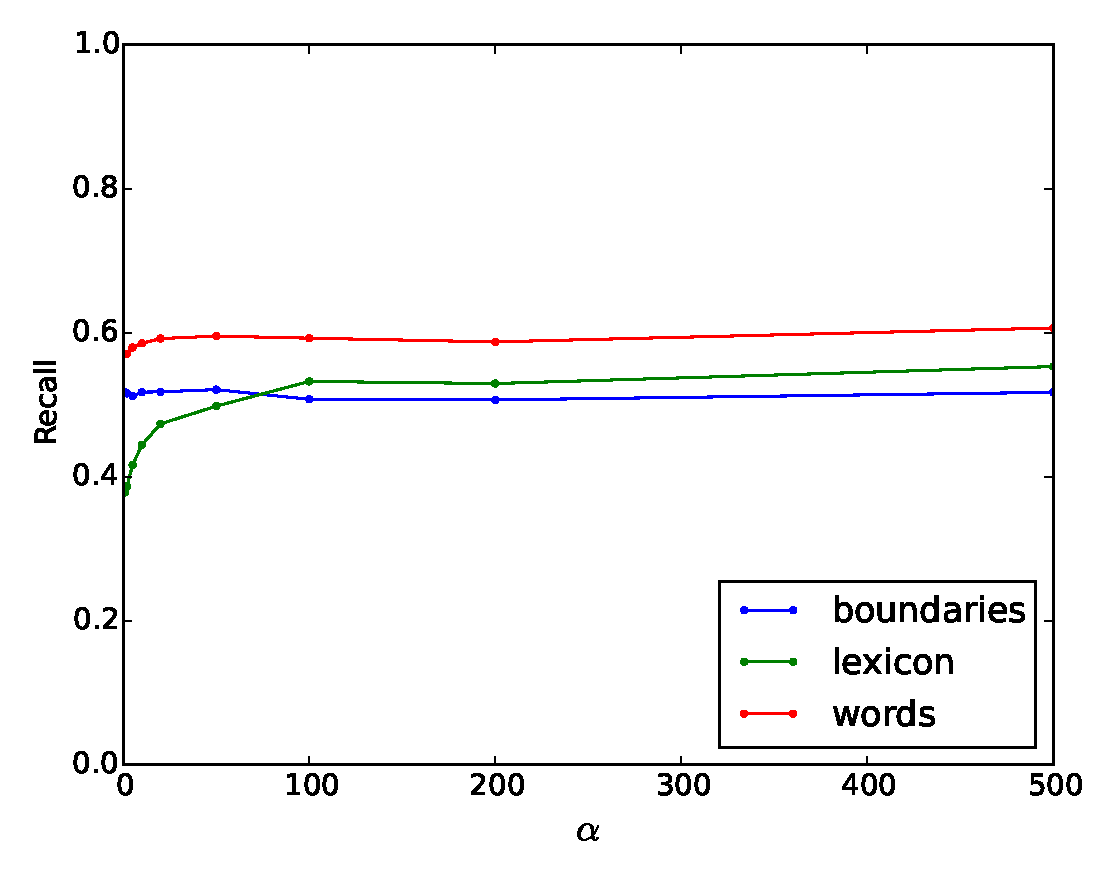
\includegraphics[width=0.47\linewidth]{images/alpha-recall}} &
\subfloat[Recall for different values of $p_\#$]{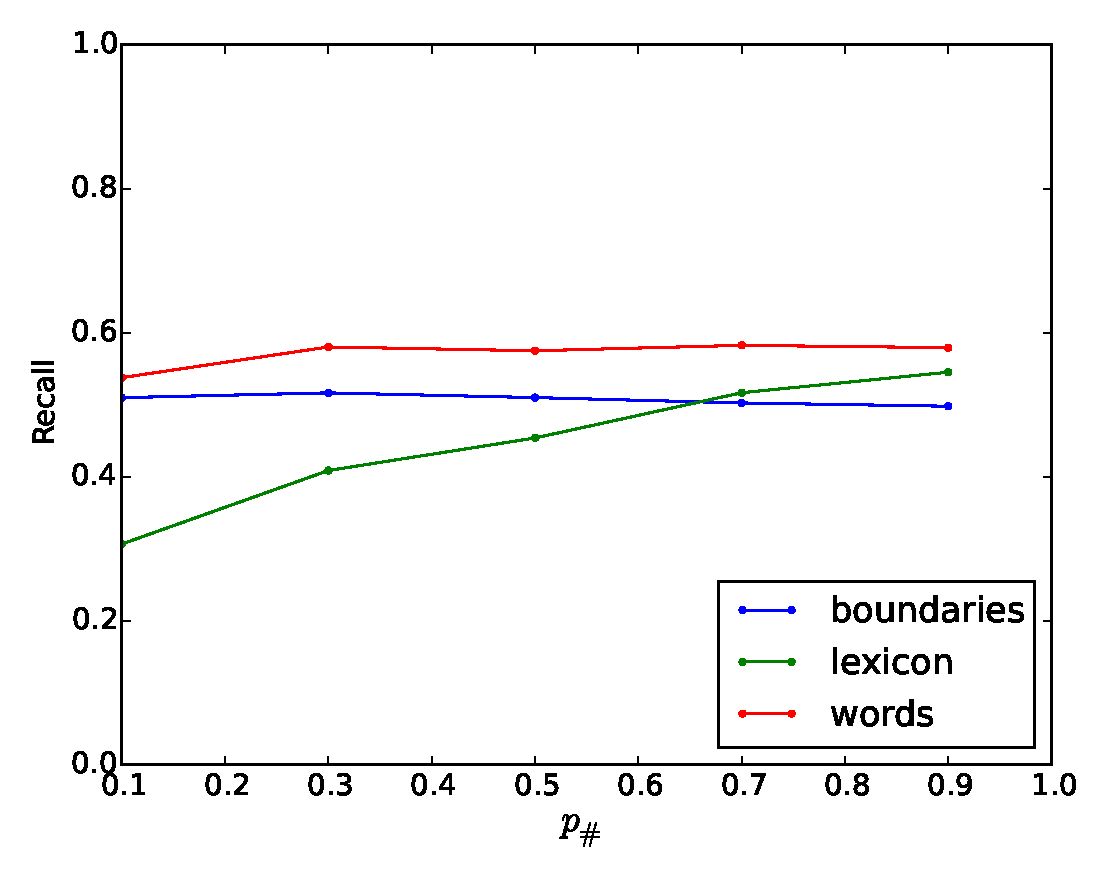
\includegraphics[width=0.47\linewidth]{images/p_dash-recall}}\\
\subfloat[$F_0$ for different values of $\alpha_0$]{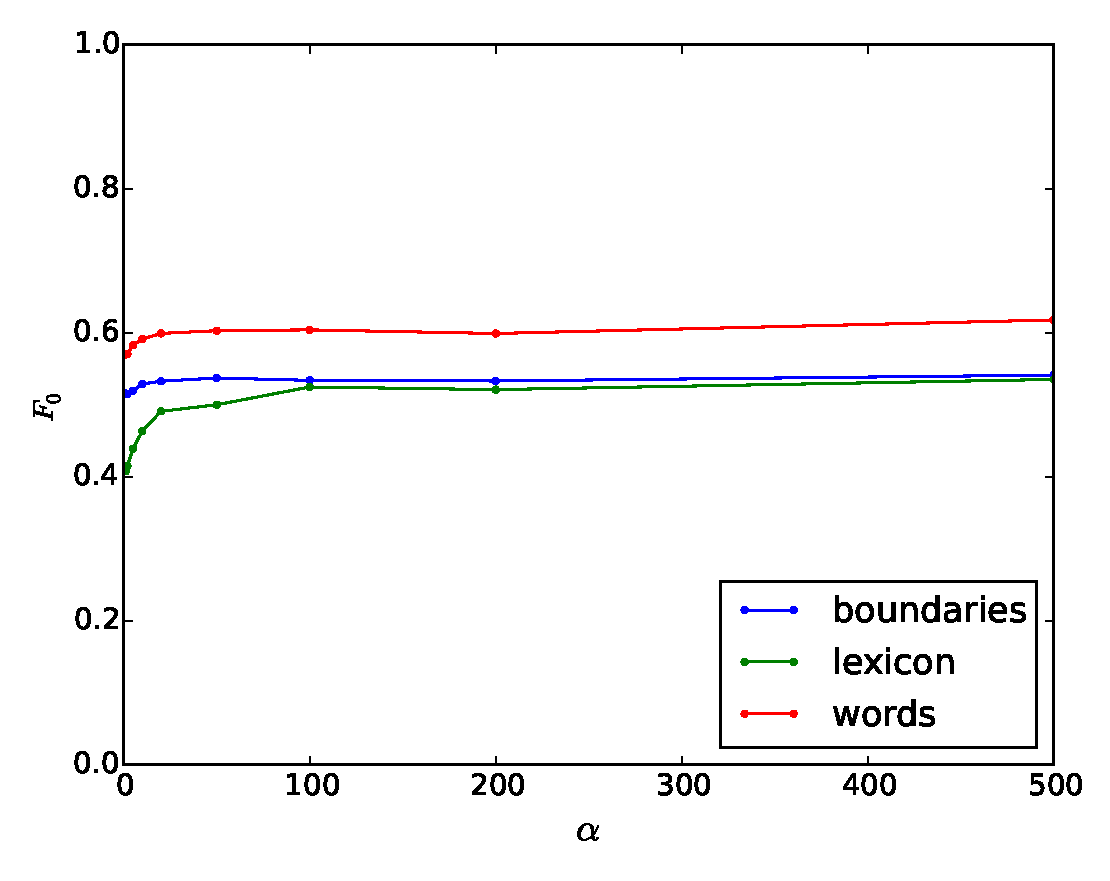
\includegraphics[width=0.47\linewidth]{images/alpha-f0}} &
\subfloat[$F_0$ for different values of $p_\#$]{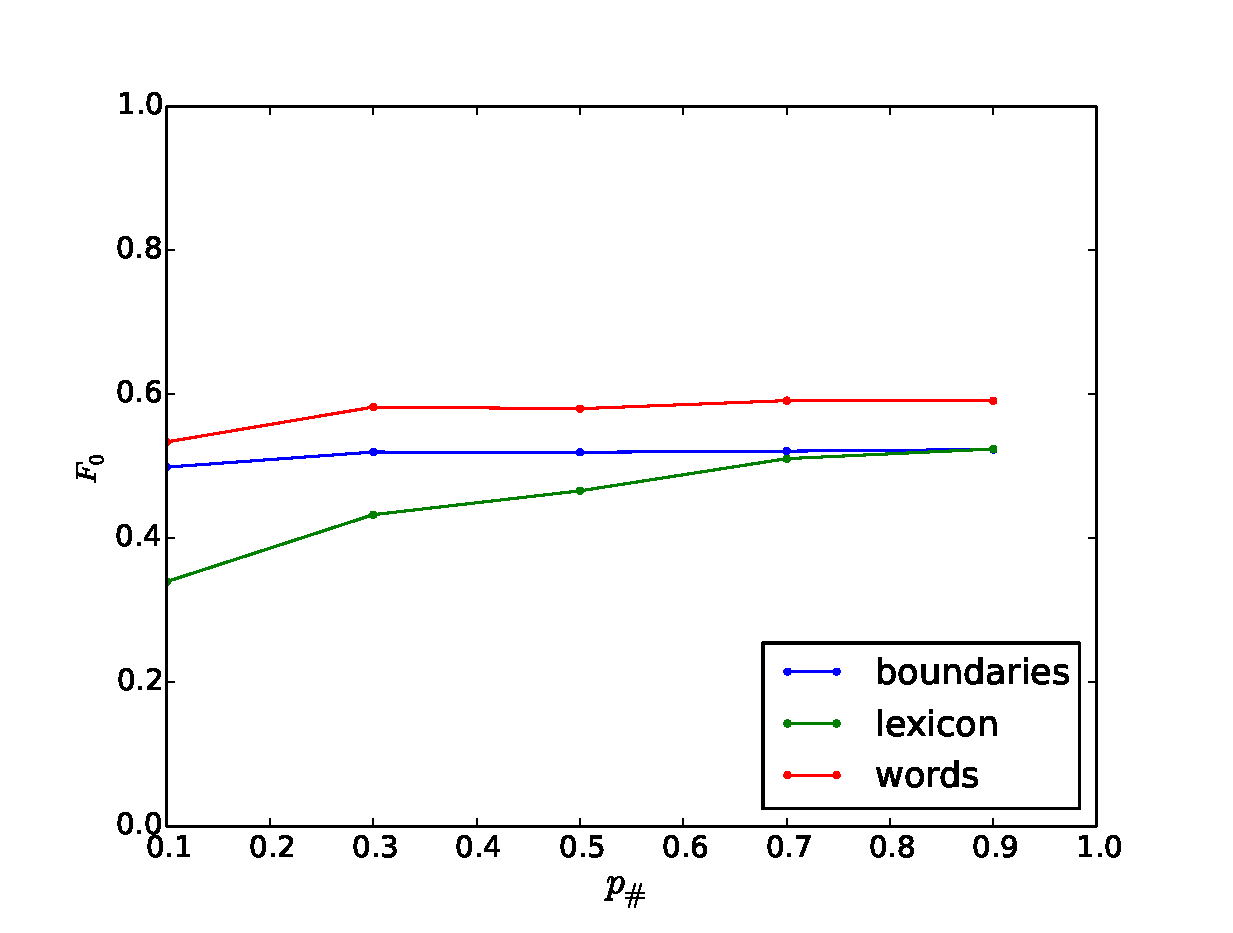
\includegraphics[width=0.47\linewidth]{images/p_dash-f0}}
\end{tabular}
\caption{The effect of different values for $\alpha_0$ and $p_\#$ on retrieval quality evaluated on words, boundaries and the lexicon.}
\label{fig:model_parameters}
\end{figure}

\subsection{Qualitative results}

To find out why the model does not perform perfectly, we must analyse the segmentation that is produces. Below are some good and bad examples.\\

\noindent\textbf{Good examples}

\begin{itemize}
\item \texttt{fid It} (actual)\\ \texttt{fid It} (retrieved)
\item \texttt{pUt It In oke} (actual)\\ \texttt{pUt It In oke} (retrieved)
\item \texttt{oke} (actual)\\ \texttt{oke} (retrieved)
\item \texttt{gIv hIm 6 kIs oke kAm an} (actual)\\ \texttt{gIv hIm 6 kIs oke kAm an} (retrieved)
\item \texttt{lUk} (actual)\\ \texttt{lUk} (retrieved)
\item \texttt{D\&t} (actual)\\ \texttt{D\&t} (retrieved)
\item \texttt{WAt 6 n9s dOgi} (actual)\\ \texttt{WAt 6 n9s dOgi} (retrieved)
\item \texttt{lEts si nQ hu goz W* D\&ts WAt 9d l9k tu no} (actual)\\ \texttt{lEtssi nQ hu goz W* D\&ts WAt 9d l9k tu no} (retrieved)
\end{itemize}

\noindent\textbf{Bad examples}

\begin{itemize}
\item \texttt{D\&ts r9t} (actual)\\ \texttt{D\&tsr9t} (retrieved)
\item \texttt{Ol r9t nQ WAt wUd yu l9k} (actual)\\ \texttt{Olr9t nQWAt wUdyul9k} (retrieved)
\item \texttt{WAt dId yu du t6de} (actual)\\ \texttt{W AtdIdy udut6de} (retrieved)
\item \texttt{WAt Els wUd yu l9k} (actual)\\ \texttt{WAtEls wUdyul9k} (retrieved)
\item \texttt{WAt Iz D\&t} (actual)\\ \texttt{WAtIzD\&t} (retrieved)
\item \texttt{wUd yu l9k D6 dOgi} (actual)\\ \texttt{wUdyul9k D6dOgi} (retrieved)
\item \texttt{k\&n yu rid 6 bUk} (actual)\\ \texttt{k\&nyu ri d6bUk} (retrieved)
\item \texttt{v*i gUd} (actual)\\ \texttt{v*igUd} (retrieved)
\end{itemize}

We see that the good examples consist mostly of very short utterances, which are arguably easier to segment than longer utterances. The bad examples consist mostly of quite long utterances, and we can clearly see that they all lack boundaries. In other words, the model undersegments these utterances.
